 \documentclass[a4paper,twocolumn,10pt]{article}
\usepackage[utf8]{inputenc}
\usepackage[spanish, es-tabla]{babel}
\usepackage[version=3]{mhchem}
\usepackage[journal=jacs]{chemstyle}
\usepackage{amsmath}
\usepackage{amsfonts}
\usepackage{amssymb}
\usepackage{makeidx}
\usepackage{xcolor}
\usepackage{lipsum}
\usepackage[stable]{footmisc}
\usepackage[section]{placeins}
%Paquetes necesarios para tablas
\usepackage{longtable}
\usepackage{array}
\usepackage{xtab}
\usepackage{multirow}
\usepackage{colortab}
\usepackage{listings}
%Paquete para el manejo de las unidades
\usepackage{siunitx}
\sisetup{mode=text, output-decimal-marker = {,}, per-mode = symbol, qualifier-mode = phrase, qualifier-phrase = { de }, list-units = brackets, range-units = brackets, range-phrase = --}
\DeclareSIUnit[number-unit-product = \;] \atmosphere{atm}
\DeclareSIUnit[number-unit-product = \;] \pound{lb}
\DeclareSIUnit[number-unit-product = \;] \inch{"}
\DeclareSIUnit[number-unit-product = \;] \foot{ft}
\DeclareSIUnit[number-unit-product = \;] \yard{yd}
\DeclareSIUnit[number-unit-product = \;] \mile{mi}
\DeclareSIUnit[number-unit-product = \;] \pint{pt}
\DeclareSIUnit[number-unit-product = \;] \quart{qt}
\DeclareSIUnit[number-unit-product = \;] \flounce{fl-oz}
\DeclareSIUnit[number-unit-product = \;] \ounce{oz}
\DeclareSIUnit[number-unit-product = \;] \degreeFahrenheit{\SIUnitSymbolDegree F}
\DeclareSIUnit[number-unit-product = \;] \degreeRankine{\SIUnitSymbolDegree R}
\DeclareSIUnit[number-unit-product = \;] \usgallon{galón}
\DeclareSIUnit[number-unit-product = \;] \uma{uma}
\DeclareSIUnit[number-unit-product = \;] \ppm{ppm}
\DeclareSIUnit[number-unit-product = \;] \eqg{eq-g}
\DeclareSIUnit[number-unit-product = \;] \normal{\eqg\per\liter\of{solución}}
\DeclareSIUnit[number-unit-product = \;] \molal{\mole\per\kilo\gram\of{solvente}}
\usepackage{cancel}
%Paquetes necesarios para imágenes, pies de página, etc.
\usepackage{graphicx}
\usepackage{lmodern}
\usepackage{fancyhdr}
\usepackage[left=2cm,right=2cm,top=2cm,bottom=2cm]{geometry}

%Instrucción para evitar la indentación
%\setlength\parindent{0pt}
%Paquete para incluir la bibliografía
\usepackage[backend=bibtex,style=chem-acs,biblabel=dot]{biblatex}
\addbibresource{references.bib}

%Formato del título de las secciones

\usepackage{titlesec}
\usepackage{enumitem}
\titleformat*{\section}{\bfseries\large}
\titleformat*{\subsection}{\bfseries\normalsize}

%Creación del ambiente anexos
\usepackage{float}
\floatstyle{plaintop}
\newfloat{anexo}{thp}{anx}
\floatname{anexo}{Anexo}
\restylefloat{anexo}
\restylefloat{figure}

%Modificación del formato de los captions
\usepackage[margin=10pt,labelfont=bf]{caption}

%Paquete para incluir comentarios
\usepackage{todonotes}

%Paquete para incluir hipervínculos
\usepackage[colorlinks=true, 
            linkcolor = blue,
            urlcolor  = blue,
            citecolor = black,
            anchorcolor = blue]{hyperref}

\usepackage{amsmath}
\usepackage{amssymb}
\usepackage{braket}
\usepackage{graphics}
\usepackage{listings}
\usepackage{xcolor}
\usepackage{framed, color}



\definecolor{codepurple}{rgb}{0.58,0,0.82}

\definecolor{bronze}{rgb}{0.8, 0.5, 0.2}
\definecolor{codegray}{rgb}{0.5,0.5,0.5}
\definecolor{antiquewhite}{rgb}{0.98, 0.92, 0.84}
\definecolor{munsell}{rgb}{0.0, 0.5, 0.69}
\definecolor{blanchedalmond}{rgb}{1.0, 0.92, 0.8}
\definecolor{cosmiclatte}{rgb}{1.0, 0.97, 0.91}
\definecolor{cobalt}{rgb}{0.0, 0.28, 0.67}

\lstdefinestyle{mystyle}{
    backgroundcolor=\color{cosmiclatte},   
    commentstyle=\color{bronze},
    keywordstyle=\color{cobalt},
    numberstyle=\tiny\color{codegray},
    stringstyle=\color{codepurple},
    basicstyle=\ttfamily\footnotesize,
    breakatwhitespace=false,         
    breaklines=true,                 
    captionpos=b,                    
    keepspaces=true,                 
    numbers=left,                    
    numbersep=5pt,                  
    showspaces=false,                
    showstringspaces=false,
    showtabs=false,                  
    tabsize=2
}


\lstset{style=mystyle}

\renewcommand{\listingscaption}{Listado}
\listoflistings

%%%%%%%%%%%%%%%%%%%%%%
%Inicio del documento%


\begin{document}
\title{\textbf{\Bbb{Proyecto Computación Concurrente}}}
\author{Cota Martínez Guillermo\\
Barriga Rosales Alan\\
Macías Gomez Jorge}


\twocolumn[
\begin{@twocolumnfalse}
\maketitle
\vspace*{-1cm}
\begin{center}\rule{0.9\textwidth}{0.1mm} \end{center}
\begin{abstract}
\normalsize Realizamos una comparación de tres algoritmos diferentes para medir el rendimiento y eficiencia de los tres, realizando la misma tarea.\\ El problema de igualar una cadena usando un algoritmo evolutivo secuencial, y dos ejecuciones concurrentes. Realizamos el análisis con casos de prueba de distinto tamaño para medir las curvas de complejidad de cada algoritmo y realizamos una análisis de tiempo y uso de CPU .\\
\begin{center}\rule{0.9\textwidth}{0.1mm} \end{center}
\vspace*{0.5cm}
\end{abstract}
\end{@twocolumnfalse}
]

\section{Objetivo}
Comparar ejecuciones secuenciales y concurrentes de un algoritmos evolutivo para igualar un string con entradas de diferentes tamaños y analizar el rendimiento de los mismos. 

\section{Marco Teórico}

%\subsection{Las redes neuronales artificiales.}
%Las redes neuronales artificiales son un modelo computacional inspirado en el comportamiento observado en su homólogo biológico. Consiste en un conjunto de unidades, llamadas neuronas artificiales, conectadas entre sí para transmitirse señales. La información de entrada atraviesa la red neuronal (donde se somete a diversas operaciones) produciendo unos valores de salida.\\
%Cada neurona está conectada con otras a través de unos enlaces. En estos enlaces el valor de salida de la neurona anterior es multiplicado por un valor de peso. Estos pesos en los enlaces pueden incrementar o inhibir el estado de activación de las neuronas adyacentes. Del mismo modo, a la salida de la neurona, puede existir una función limitadora o umbral, que modifica el valor resultado o impone un límite que no se debe sobrepasar antes de propagarse a otra neurona. Esta función se conoce como función de activación.


\subsection{Algoritmos evolutivos}
Se pretende presentar un resumen de algunos de los distintos algoritmos evolutivos, pues a pesar de que tomamos uno, existen varios tipos.

\subsubsection*
{Colonia de abejas artificiales}

Este algoritmo se basa en la optimización del comportamiento de los enjambres de abejas en busca de miel donde la colonia consta de tres grupos de abejas: empleadas, exploradores y en espera. Se asume que hay solo una abeja empleada para cada fuente de alimento. En otras palabras, el número abejas empleadas en la colonia es igual al número de fuentes de alimentos alrededor de la colmena. Las abejas empleadas van a su fuente de alimento, vuelven a la colmena y danzan en esta área. La abeja empleada cuya fuente de alimentos ha sido abandonada se convierte en exploradora y empieza la búsqueda de nuevas fuentes de alimentación. Las abejas en espera observan las danzas de las abejas empleadas y escogen las fuentes de alimentos dependiendo de las danzas.
\begin{figure}[h]
    \centering
    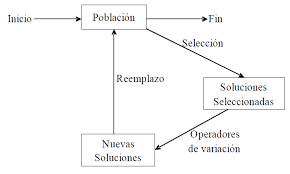
\includegraphics[scale=0.45]{abejas.png}
    \caption{Colonia de Abejas}
    \label{fig:mesh1}
\end{figure}

\subsubsection*{Colonia de hormigas}

Estos algoritmos, que están basados en una colonia de hormigas artificial, son agentes computacionales que trabajan de manera conjunta para poder comunicarse a través de rastros de feromonas artificiales. En cada iteración del algoritmo cada hormiga construye una solución al problema a través de un grafo. Cada arista representa las posibles opciones que el
insecto puede tomar.
La idea general es identificar caminos cortos y caminos largos como el camino inferior es más corto que el superior, muchas más hormigas transitarán por éste durante el mismo periodo de tiempo. Esto implica que en el camino más corto se acumula más feromona mucho más rápido.
Después de cierto tiempo, la diferencia en la cantidad de feromona en los dos caminos es lo suficientemente grande para influenciar la decisión de las nuevas hormigas que entren a recorrer estas vías.
\begin{figure}[h]
    \centering
    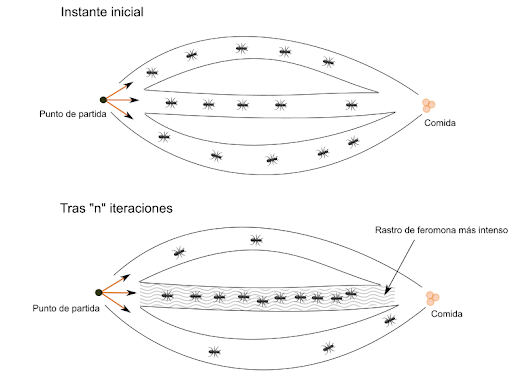
\includegraphics[scale=0.45]{hormigas.png}
    \caption{Colonia de Hormigas}
    \label{fig:mesh1}
\end{figure}
\subsubsection*{Búsqueda armónica}
En el modelo básico de Búsqueda Armónica(BA), cada solución candidata es considerada una “armonía”, y es representada por un vector n-dimensional. La población inicial de las soluciones candidatas es aleatoriamente inicializada y almacenada dentro de una memoria (Harmony Memory “HM”). De esta manera, una nueva solución es generada a partir de uno de los elementos contenidos en HM, a través de una operación de re-inicialización aleatoria o mediante una operación de ajuste de “tono” de un vector contenido en ella. Finalmente, la HM es actualizada mediante la comparación de la nueva solución candidata y el peor de los vectores contenidos en HM, si esta es mejor, remplazará el lugar del vector dentro de la memoria, de lo contrario no existirá cambio alguno. Este proceso se realiza hasta cumplir el criterio de paro. La forma básica del algoritmo BA consiste en tres etapas: inicialización, improvisación de nuevas armonías (generación de nuevas soluciones) y la actualización de la memoria (HM). 

\subsubsection*{Evolución diferencial}

La Evolución Diferencial (ED) es un método de optimización perteneciente a la categoría de computación evolutiva, aplicado en la resolución de problemas complejos. Al igual que otros algoritmos de esta categoría, la ED mantiene una población de soluciones candidatas, las cuales se recombinan y mutan para producir nuevos individuos los cuales serán elegidos de acuerdo al valor de su función de desempeño. Lo que caracteriza a la ED es el uso de vectores de prueba, los cuales compiten con los individuos de la población actual a fin de sobrevivir.

El algoritmo asume que las variables del problema a optimizar están codificadas como un vector de números reales. La longitud de estos vectores (n)es igual al número de variables del problema, y la población está compuesta de NP (Número de padres)vectores. Se define un vector $ {\displaystyle x_{p}^{g}}{\displaystyle x_{p}^{g}}$, en donde p es el índice del individuo en la población (p = 1...NP) y g es la generación correspondiente. Cada vector está a su vez compuesto de las variables del problema ${\displaystyle x_{p,m}^{g}}{\displaystyle x_{p,m}^{g}}$, en donde m es el índice de la variable en el individuo (m = 1...n).

Se asume que el dominio de las variables del problema está restringido entre valores mínimos y máximos ${\displaystyle x_{m}^{min}}{\displaystyle x_{m}^{min}} y {\displaystyle x_{m}^{max}}{\displaystyle x_{m}^{max}}$, respectivamente.

ED se compone básicamente de 4 pasos:
\begin{itemize}
    \item Inicialización
    \item Mutación
    \item Recombinación
    \item Selección

\end{itemize}



\subsection*{Algoritmos Genéticos}

Los algoritmos genéticos son una técnica de búsqueda que permite optimizar funciones. Para ello requieren:

\begin{itemize}
    \item Codificar soluciones como cromosomas
    \item Una función de evaluación
    \item Método para inicializar la población de cromosomas.
    \item Operadores para obtener a la siguiente generación. Ej: mutación, cruza y operadores específicos de dominio.
    \item Asignaciones a los parámetros.
\end{itemize}

Procedimiento para la búsqueda genética:
\begin{verbatim}

Inicializar población:
Ordenar población según función de evaluación
While criterio de paro do:
        Seleccionar uno o más padres aleatoriamente, los mejores con mayor probabilidad.
        Aplicar operadores para producir hijos
        Insertar hijos/reemplazar padres
return Mejor individuo
\end{verbatim}





\section{Elección del AEB a
desarrollar}


Como podemos tenemos una gran variedad de opciones para resolver nuestro problema, sin embargo también podemos observar que cada uno de los métodos descritos anteriormente tiene condiciones que los hacen óptimos para resolver distintos tipos de problemas. Una vez analizado nuestro problema nosotros optamos por desarrollar un algoritmo genético pues nuestro proyecto a grandes rasgos buscara, de una palabra, conocer sus análogas que sean similares, es decir, la manera "más natural" en el que puede ser interpretado es con inicializar una lista de palabras aleatorias seleccionar alguna e ir la cambiando (lo vemos como un proceso de mutación o cruza), para que vaya evolucionando hasta llegar al objetivo que es obtener el símil. 

Por lo anteriormente expuesto podemos observar que el método más simple consiste en atacar nuestro problema con la implementación de un algoritmo genético.


\section{Planteamiento del problema y Metodología}

Buscamos resolver el siguiente problema:\\ 
Dada una cadena de texto, inicializar una lista de cadenas aleatorias de la misma longitud para evolucionarlas a través de generaciones y lograr el parecido más próximo o la igualdad del objetivo.\\
Esto es que se inicializará una \textit{generación de genes o cromosomas}, se seleccionará alguna y se mutará o cruzará con otro cromosoma para ir evolucionando la lista de palabras a otra lista que tenga palabras más similares a la palabra objetivo.\\
Dado un número de \textit{población} por generación (es decir, cuántos candidatos habrá cada generación), inicializaremos ese número de candidatos aleatorios, y ordenamos de mejor \textit{aptitud} a peor aptitud (aquí aptitud es la función error que indica la suma de carácteres distintos entre una cadena y el objetivo).\\
\subsection*{Operadores genéticos}
En nuestro algoritmo tenemos dos: mutación y cruza.\\
Explicaremos cómo se hace la mutación. Dado un cromosoma (gen) aleatorio, se selecciona un octavo de sus carácteres y se intercambian por algún otro carácter. Por otro lado, la cruza significa elegir dos cromosomas y seleccionar la mitad de alguno de los dos para el cromosoma hijo y la otra mitad del otro gen, de esta manera, el gen hijo tendrá la mitad de los genes de un cromosoma y la otra del otro.
\subsection{Selección de cromosomas para operar}
En cada generación, existen genes que tienen mejor aptitud que otros, es decir, si pensamos en su analogía con la naturaleza, lo que representaría la aptitud sería la capacidad de supervivencia de cada gen, entonces para hacer efectivo el similar natural, en cada generación, aquellos que tienen tendencia a mutar, serán aquellos que tengan mejor aptitud, de igual manera, en la cruza, los padres serán probablemente aquellos genes que tengan la mejor aptitud. Para esto se definió un parámetro llamato \verb|pelite| que significa la probabilidad de que el mejor gen sea elegido. La elección del gen a mutar/padre para cruzar es el siguiente: Se inicializa una variable que va contando el índice a elegir de la lista ordenada de los genes de la generación de mejor a peor aptitud y se corre un número aleatorio uniforme entre 0 y 1, si aquel número es menor que \verb|pelite|, entonces el índice indica el cromosoma a elegir, en caso contrario, en índice aumenta en uno (se la juega el segundo mejor cromosoma) y se vuelve a correr el experimento del número aleatorio, nuevamente se verifica si es menor al parámetro \verb|pelite| y en caso contrario, se seguirá al tercer mejor gen y así sucesivamente hasta que se eliga un gen. Como se puede intuir, esto corresponde a una variable aleatoria $X \sim Geom(\verb|pelite|)$.
\subsection{Algoritmo para solucionar el problema}
Para nuestro ejercicio, tenemos tres elementos: operadores genéticos, generación a evolucionar e iteraciones de evolución. Entonces el algoritmo consiste en lo siguiente:
\begin{itemize}
    \item Se inicializa una primera generación aleatoria.
    \item Para cada nuevo gen de la siguiente generación se elige un operador genético y se aplica (Aquí es donde sucederá la concurrencia en nuestros algoristmos)
    \item Con la nueva generación, se repite el paso anterior, ahora eligiendo operadores genéticos para esta generación y se repite hasta completar cierto número de iteraciones.
\end{itemize}
\subsection{Cuatro algoritmos}
Se procedió a realizar la evolución de las generaciones con cuatro algoritmos listadas a continuación así como su posición en el código \verb|Genético.py|:
\begin{itemize}
    \item Secuencial (Lineas 125-244)\\
    Este modelo es la implementación sin concurrencia para medir su rapidez ante los siguientes.
    \item Usando \verb|mp.Pool()| (Líneas 249-408)\\
     Se usaron 8 procesadores y el mapeo \verb|mp.Pool().starmap()| que toma como parámetros la función 'Crear hijos' y una lista iterable con los parámetros, en el cual la función 'Crear hijos' devolverá un cromosoma de la nueva generación, haciendo que se vayan creando tareas para cada uno de los procesos.\\
    \item Usando \verb|mp.Process()| (Líneas 415-579)
    Usando los procesos, para cada generación, se dividió la tarea de generar cromosomas en distintos procesos. La diferencia entre este y el secuencial, es que al momento en que se procede a la obtención de cada nueva generación cada cromosoma que se iba a crear (ya sea por mutación o cruza), se realizo por un proceso distinto, es decir si población=20, entonces en cada generación, al momento de crear los cromosomas, cada cromosoma es creado por un proceso (en total se crean 20 procesos) y el proceso será el encargado de elegir el operador genético así como su creación, después se manda al proceso padre mediante una \verb|mp.Manager().Queue()|
    \item Usando \verb|mp.Process()| Segundo método (Líneas 585-759):\\
    Es similar al primer método, sin embargo, recordemos que el anterior hace uso de un proceso por cada cromosoma de la población, mientras que este hace 4 procesos en donde se divide la carga de trabajo de la creación de genes en cada generación, es decir, si población=20, entonces se procede a crear 4 procesos y cada proceso está encargado de crear 5 cromosomas. De igual manera, este método usa \verb|mp.Manager().Queue()|.\\
    
   
\end{itemize}

\section{Resultados}


Para probar el algoritmo se usó el texto de referencia conocido como Lorem Ipsum, se usaron dos formatos de este archivo: Lorem Ipsum parcial (Primeras 1000 carácteres) y completo (92551 carácteres). Así como se procedio a probar con distintos parámetros para medir la eficiencia variando las poblaciones en [8,20,200,1000] y 500 iteraciones para cada uno.


\begin{table}[h]
\resizebox{0.9\columnwidth}{!}{
\begin{tabular}{ lllll } 
     &             & \multicolumn{2}{l}{Lorem Parcial}&       \\ \hline
Pob. & Secuencial: & Concurrente1:  & Concurrente2:  & Pool:   \\ \hline
8    & 0.998       & 7.83           & 7.873          & 8.114   \\ \hline
20   & 2.566       & 30.08          & 11.963         & 15.5    \\ \hline
200  & 24.79       & NA             & 16.999         & 70.661  \\ \hline
500  & 65.571      & NA             & 25.344         & 173.524 \\ \hline
1000 & 131.709     & NA             & 34.276         & 313.812
\end{tabular}}
\caption{Muestra los resultados para Lorem Ipsum Parcial, para los primeros 1,000 carácteres y 500 iteraciones cada uno.}
\end{table}

Como podemos observar, en poca población, en un principio el algoritmo secuencial es más rápido que los que utilizan concurrencia y paralelismo, esto se cree que se debe a el pequeño tiempo que elapsa al crear un proceso nuevo y a la sincronización de los procesos. Sin embargo, conforme avanza el número de cromosomas por generación, es decir aumentamos el parámetro población, se alcanza un mejor desempeño para el método Concurrente 2.\\
Vamos a analizar el porqué pasa esto:
\begin{itemize}
    \item \textbf{Secuencial vs. Concurrente 1:} Para el primer método de concurrencia, recordemos que en cada generación se tiene la creación de un proceso para cada gen, esto quiere decir que en cada generación crea tantos procesos como cromosomas en la población. Entonces el proceso de creación para cada proceso puede llegar a ser tardado, más tardado incluso que el hecho de hacerlo secuencialmente, pues el realizarlo de esta manera no gasta tiempo en crear el proceso así como no hay tiempo de espera para su final sincronización con el proceso padre. Esto también se puede deber a que realmente el proceso de usar un operador genético (mutar o cruzar) no lleva muchos recursos con un un objetivo tan pequeño (1000 carácteres). Además no se experimentó con poblaciones más grandes que 20 pues implicaría la creación de muchos procesos, tarea la cuál, provoca problemas computacionales y terminaron atorando el ordenador.
    
    \item \textbf{Secuencial vs. Concurrente 2:} Este es el mejor modelo en su desempeño, pues en lugar de separar un proceso para cada gen, decide dividir la tarea de creación de cromosomas en pocos procesos, los cuales en este caso fueron 4 procesos para cada generación que se repartieron entre cada uno, un cuarto de la carga del trabajo, reduciendo considerablemente el tiempo de ejecución, y el hecho de que el número de procesos no varía, se pudo implementar para poblaciones hasta de 1000.
    
    \item \textbf{Secuencial vs. Pool} El funcionamiento del método Pool en python complica la mejora del tiempo de ejecución en este caso, pues se crea una tarea para cada iterable de los parámetros que recibe \verb|mp.Pool().starmap()|, enseguida para cada tarea: Se serializa la tarea y el valor de retorno (se puede pensar como un \verb|pickle.dumps()|), se deserializa la tarea y el valor de retorno (se puede pensar como un \verb|pickle.loads()|), se gasta un tiempo considerable esperando a los \verb|Locks| que genera la función y la sincronización para poner y leer datos de dichas tareas. Por lo tanto, resulta costoso en cuestión de tiempo.
\end{itemize}
Enseguida se pasó al siguiente experimento con el texto completo, y sus resultados:
\begin{table}[h]
\resizebox{0.9\columnwidth}{!}{
\begin{tabular}{lllll}
     &             & \multicolumn{2}{l}{Lorem Completo}&       \\ \hline
Pob. & Secuencial: & Concurrente1:  & Concurrente2:  & Pool:   \\ \hline
8    & 102.490       & 32.693         & 32.893         & 107.840    \\ \hline
20   & 252.366       & 92.239        &  42.118       & 469.007   \\ \hline
200  & 2442.693      & NA             & 156.520         & 5316.464  \\ \hline
\end{tabular}}
\caption{Muestra los resultados para Lorem Ipsum Completo, con 92551 carácteres y 500 iteraciones cada uno.}
\end{table}
Podemos ver algunas similitudes con la primera tabla, aunque cabe recalcar ahora la eficacia del primer método de concurrencia, que en este caso sí garantiza una mejor aproximación al problema de mejorar la velocidad de ejecución. Ahora bien, si es mejor que su desempeño del primer ejemplo, es nuevamente superado con creces por el segundo método, esto nos da indicios de que no siempre es buena idea preferir la creación de muchos procesos frente a la creación de menos procesos que se dividan las tareas. Y similarmente al primer caso, el método Pool resulta ineficaz e incluso más lento que el secuencial. El aumento de margen de velocidad frente al algoritmo sin concurrencia se debe a que en este caso ya se tienen 92551 carácteres que mutar/cruzar en cada generación, por lo tanto cada gen creado tiene que usar más recursos computacionales para su creación, lo que lleva a que cada proceso del primer método de concurrencia sea eficaz, pues el tiempo que se tarda cada proceso en ser creado, se compensa con la velocidad ganada en ejecutar tareas que requieren más recursos computacionales.\\
Ahora, haremos una comparativa con el índice de proporción de velocidades para cada método con respecto la velocidad secuencial.


\begin{table}[h]
\resizebox{0.9\columnwidth}{!}{
\begin{tabular}{ lllll } 
     &             & \multicolumn{2}{l}{Tiempo Secuencial/ Tiempo Modelo}&       \\ \hline
Pob. & Archivo & Concurrente1:  & Concurrente2:  & Pool:   \\ \hline
8    & Lorem Parcial  & 0.12           & 0.12          & 0.13   \\ \hline
20   & Lorem Parcial  & 0.08          & 0.21         & 0.16    \\ \hline
200  & Lorem Parcial  & NA             & 1.45         & 0.35  \\ \hline
500  & Lorem Parcial  & NA             & 2.58         & 0.37 \\ \hline
1000 & Lorem Parcial  & NA             & 3.8         & 0.41 \\ \hline
8    & Lorem Completo  & 3.13           & 3.11          & 0.95   \\ \hline
20   & Lorem Completo  & 2.73          & 5.99         & 0.53    \\ \hline
200  & Lorem Completo  & NA             & 15.60         & 0.45  \\ 
\end{tabular}}
\caption{Proporción entre el tiempo de ejecución del modelo secuencial frente a los distintos modelos}
\end{table}
Como podemos ver, el segundo modelo concurrente resulta sobresaliente logrando en la tarea de igualar la cadena predicción con el objetivo con respecto a su tiempo de ejecución.\\
En cuanto al problema, los parámetros que hayaron la solución con un margen de error de 3 (se debe a que existen carácteres en el archivo no compatibles con el programa) fueron para Lorem Ipsum parcial: \\
Población de 200 alrededor de la iteración 350.\\
Con población de 500 alrededor de la iteración 300.\\
Con población 1000 alrededor de la iteración 250.\\
Para poblaciones menores no se llegó a la solución en 500 iteraciones.\\
Por otro lado, para Lorem Ipsum, debido a la dificultad del problema, no se llegó en ningún experimento a la solución siendo el mejor resultado con población 200 llegando a un error de un tercio del texto. 

\subsection{Uso del CPU}

 Para comparar cada uno de los procesos, realizamos una ejecución cronometrada con cada uno de los modelos, y analizamos el uso de CPU durante el proceso durante los primeros segundos con ayuda de esta función 

\begin{lstlisting}[language=Python]
    
def cpu_usage(q,finish):
    '''
    Funcion que monitorizara el uso de los CPUs mientras
    una bandera auxiliar lo indique asi hasta un maximo de 500 registros
    donde cada registro se toma cada 0.15 fracción de segundo.
    ------------------------------------------
    :param q mp.Queue: Cola donde se guardará el uso de los procesadores
    :param finish mp.Value: Booleano que indicará cuando detener el registro
                        de los datos.
    '''
    usage = []
    max_count = 500
    i = 0
    while not finish.value and i<max_count:
        i+=1
        time.sleep(0.15)
        usage.append(
        psutil.cpu_percent(percpu=True))
    q.put(usage)
    return
\end{lstlisting}

Esto se hizo de igual manera de forma concurrente para analizar los procesos al mismo tiempo que se ejecutaban. Esto se hizo en una computadora con 8 procesadores físicos y los gráficos se anexan al final del documento, adicionalmente, se pueden encontrar más gráficos en la siguiente liga: \href{https://github.com/Equipo-Alfa-Lobo-Dinamita/LCD-CC-2021-I/tree/main/Proyecto/Plots}{Repositorio Github}

\section{ Conclusiones }
Como podemos ver, usar concurrencia reduce el tiempo de ejecución del programa, nos permite un mejor aprovechamiento de los recursos, en especial de la CPU, ya que pueden aprovechar las fases de entrada-salida de unos procesos para realizar las fases de procesamiento de otros. De la misma forma existen contras, al incrementar los procesos, es decir, la concurrencia, el programa volvía a ver su velocidad reducida, es un ejemplo de la Ley de Amdahl y ley de Gustafson. Que nos quieren decir que toda tarea tiene un punto máximo de velocidad que esta fijo según la parte no paralelizable del algoritmo, podemos concluir entonces, que es necesario tener un balance entre la cantidad de procesadores y las tareas realizadas por cada uno. 




\pagebreak


% This section should spread over both columns
\onecolumn
\section{Apéndices}
\subsection{Gráficas de uso de los CPUs}
A continuación se muestran los gráficos obtenidos del monitoreo del uso de los CPUs para los cuatro modelos propuestos.
\begin{figure}[H]
    \centering
    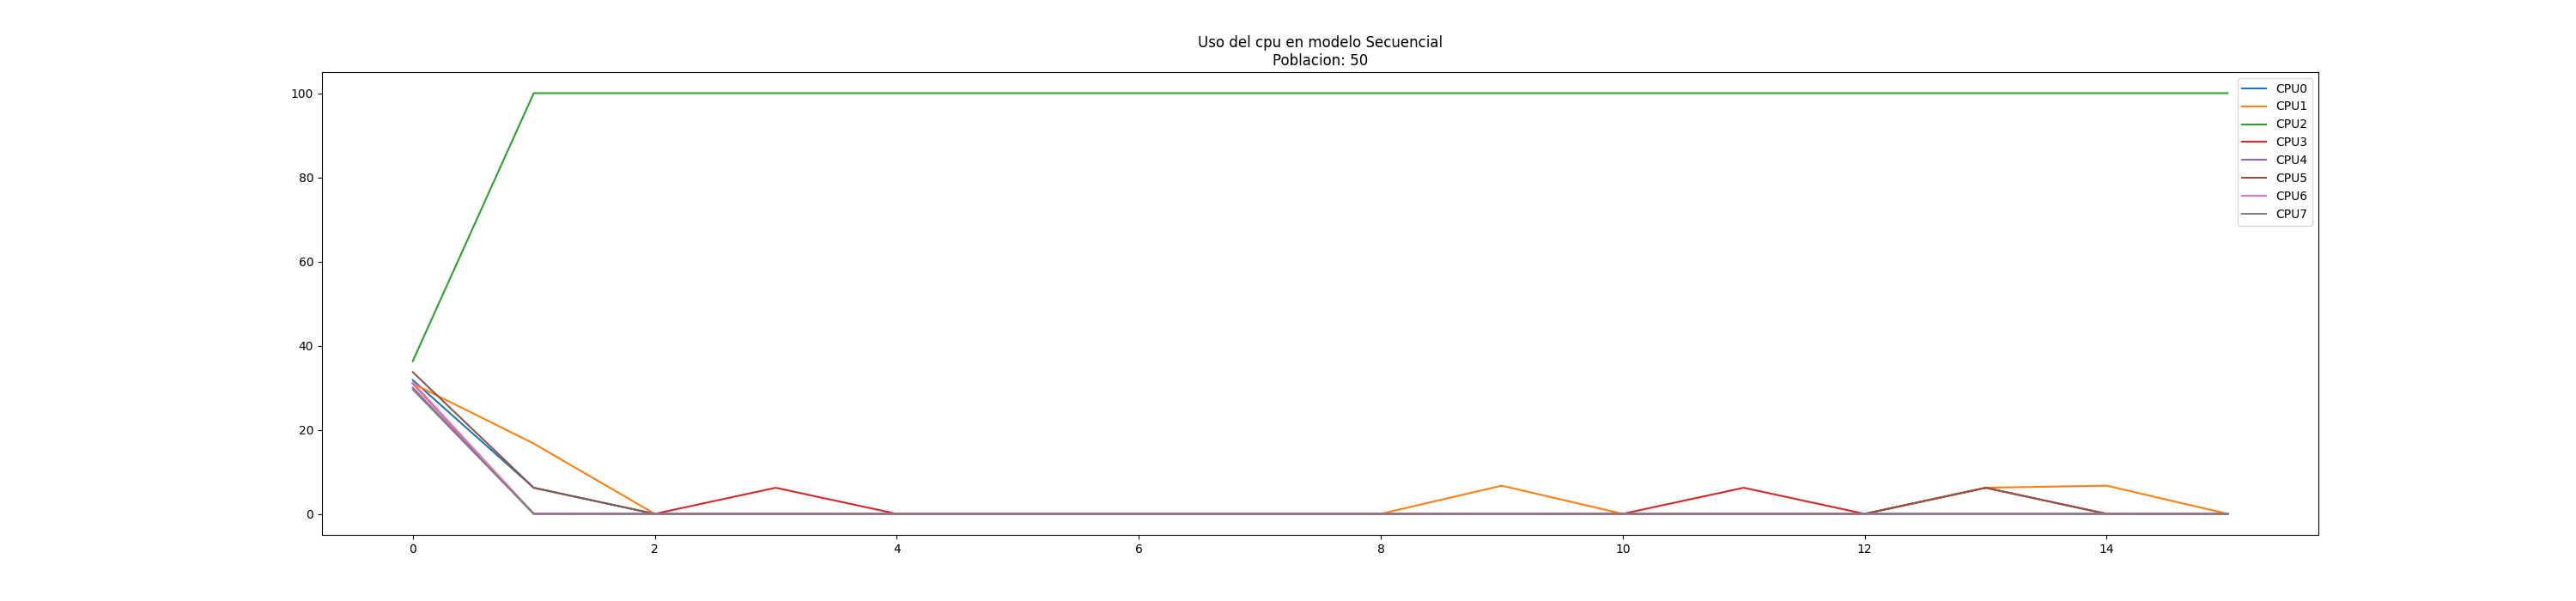
\includegraphics[width=\linewidth]{Plots/ModeloSecuencial_Poblacion50.png}
    \caption{Uso de recursos de modelo secuencial}
\end{figure}
Como podemos ver en este ejemplo, el uso de código de forma secuencial, genera el uso de un solo procesador, que en un principio, supone el uso de un solo procesador destinado al uso de Python, sin embargo, en la siguiente gráfica, que monitorea el uso de recursos durante más tiempo, se observa que esto no es cierto, pues a la larga va cambiando de un procesador a otro, siendo aún secuencial:
\begin{figure}[H]
    \centering
    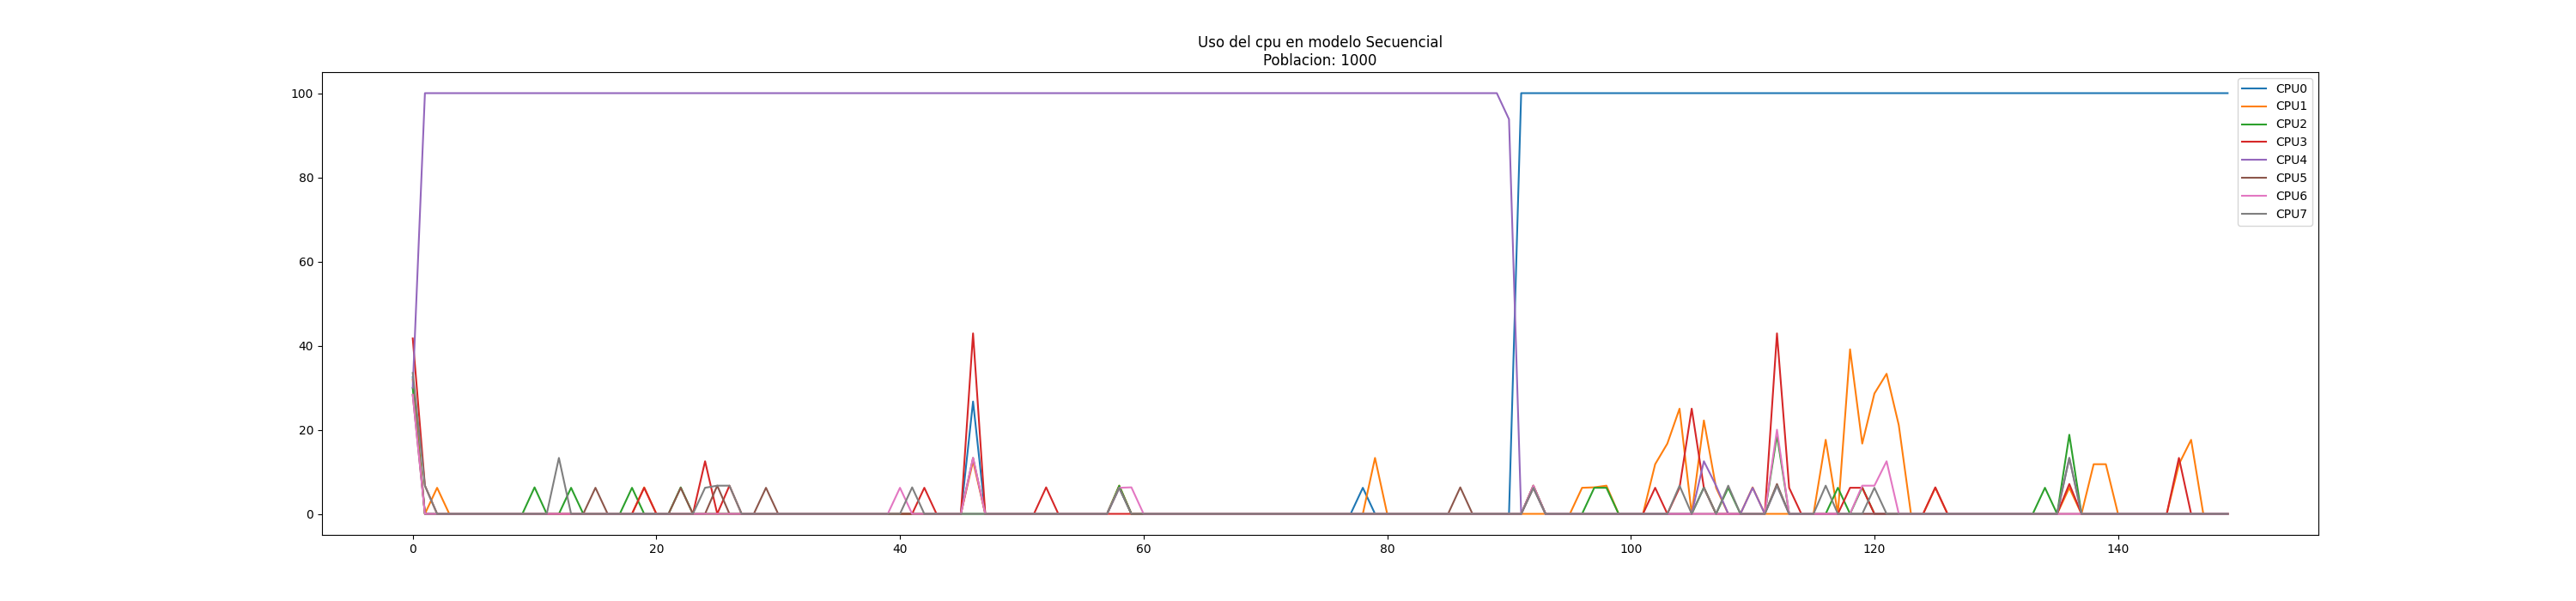
\includegraphics[width=\linewidth]{Plots/ModeloSecuencial_Poblacion1000.png}
    \caption{Uso de recursos de modelo secuencial con poblacion=1000}
\end{figure}
Ahora, veamos cómo es el uso de recursos para el método \verb|mp.Pool()|
\begin{figure}[H]
    \centering
    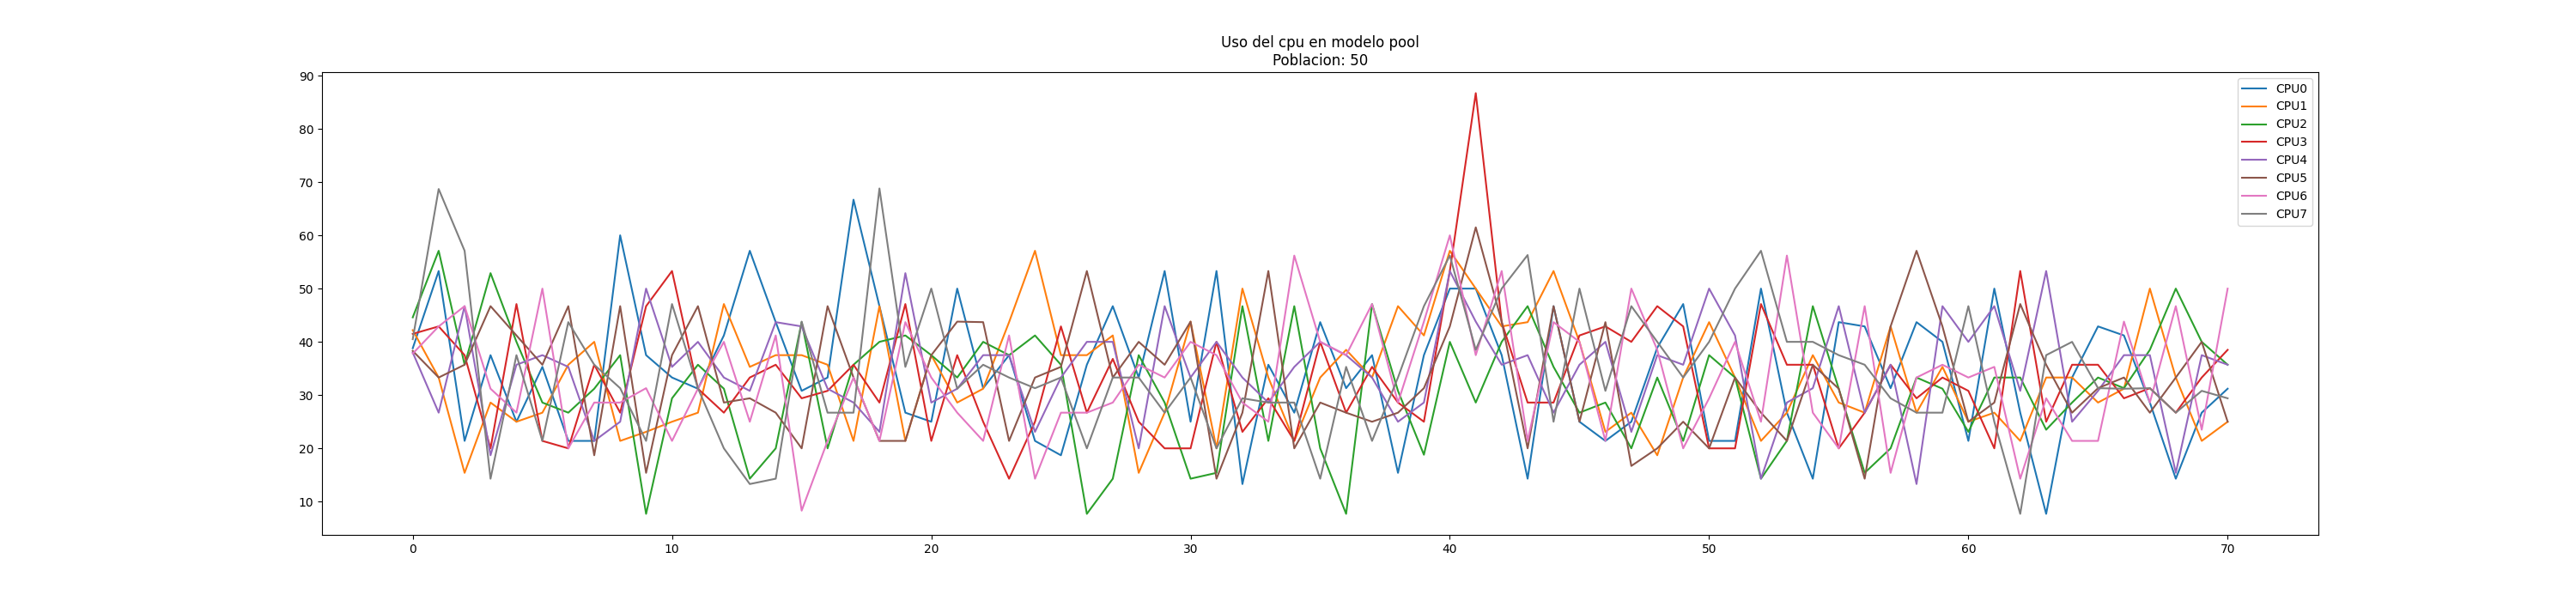
\includegraphics[width=\linewidth]{Plots/Modelopool_Poblacion50.png}
    \caption{Uso de recursos de modelo Pool}
\end{figure}
Así se ve el uso de múltiples procesadores para cumplir la tarea, esto es similar en el uso de \verb|mp.Process()|, sin embargo en el primer método se ve afinidad por usar un procesador para una mayor carga de trabajo.
\begin{figure}[H]
    \centering
    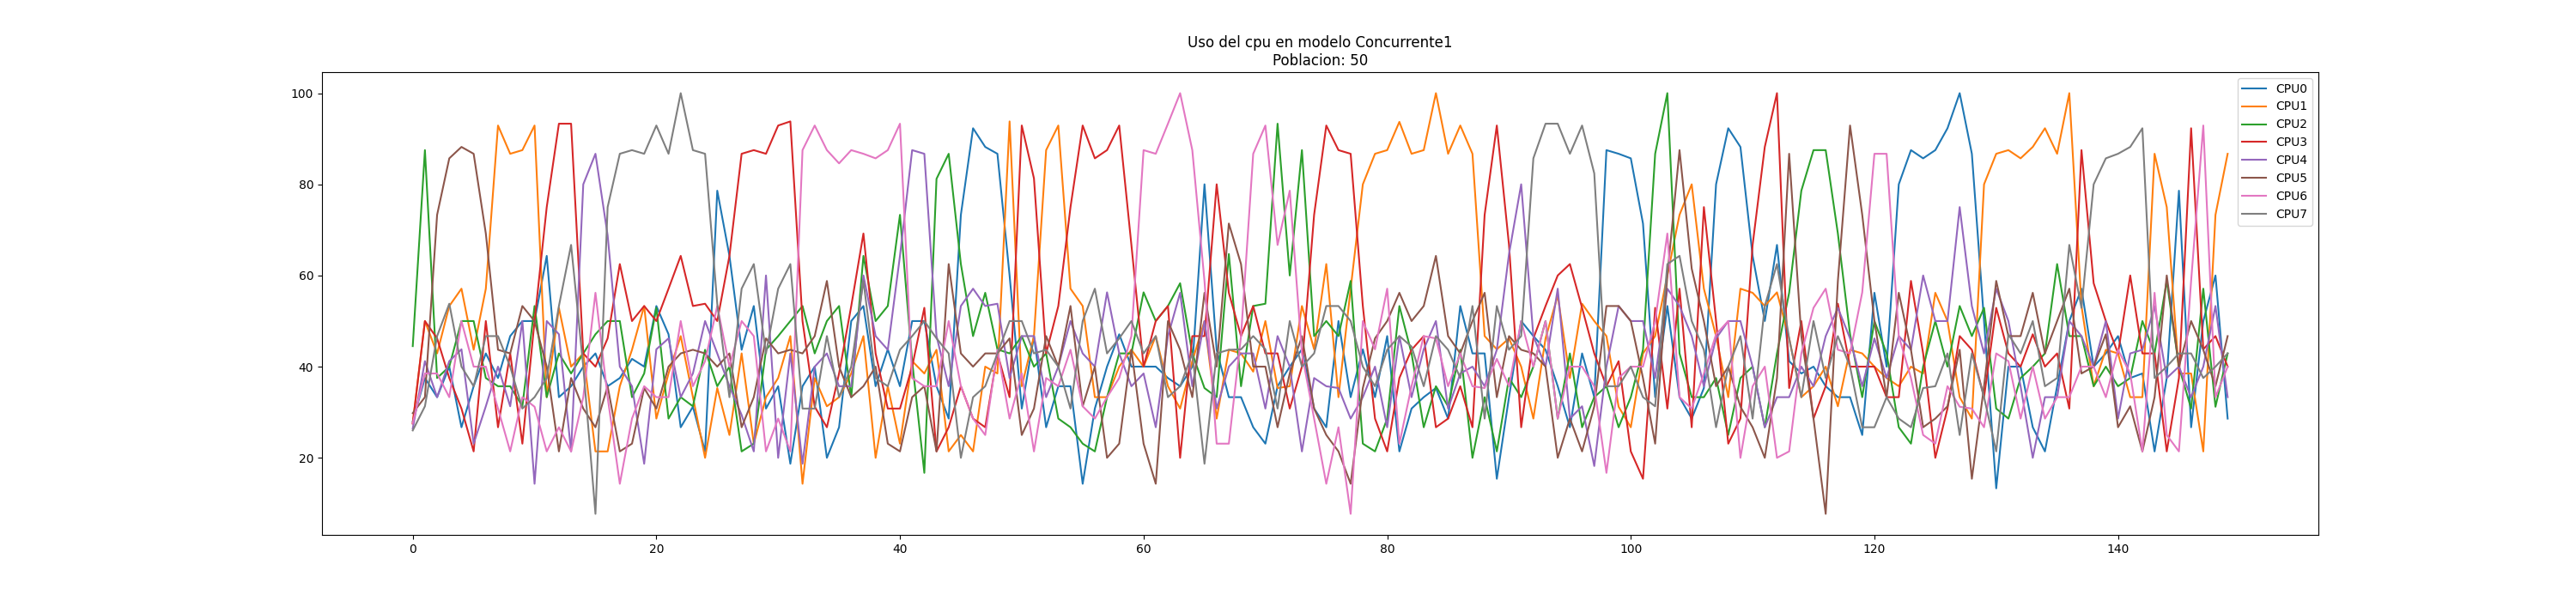
\includegraphics[width=\linewidth]{Plots/ModeloConcurrente1_Poblacion50.png}
    \caption{Uso de recursos de modelo Concurrente1 (1 proceso para cada cromosoma hijo)}
\end{figure}
\begin{figure}[H]
    \centering
    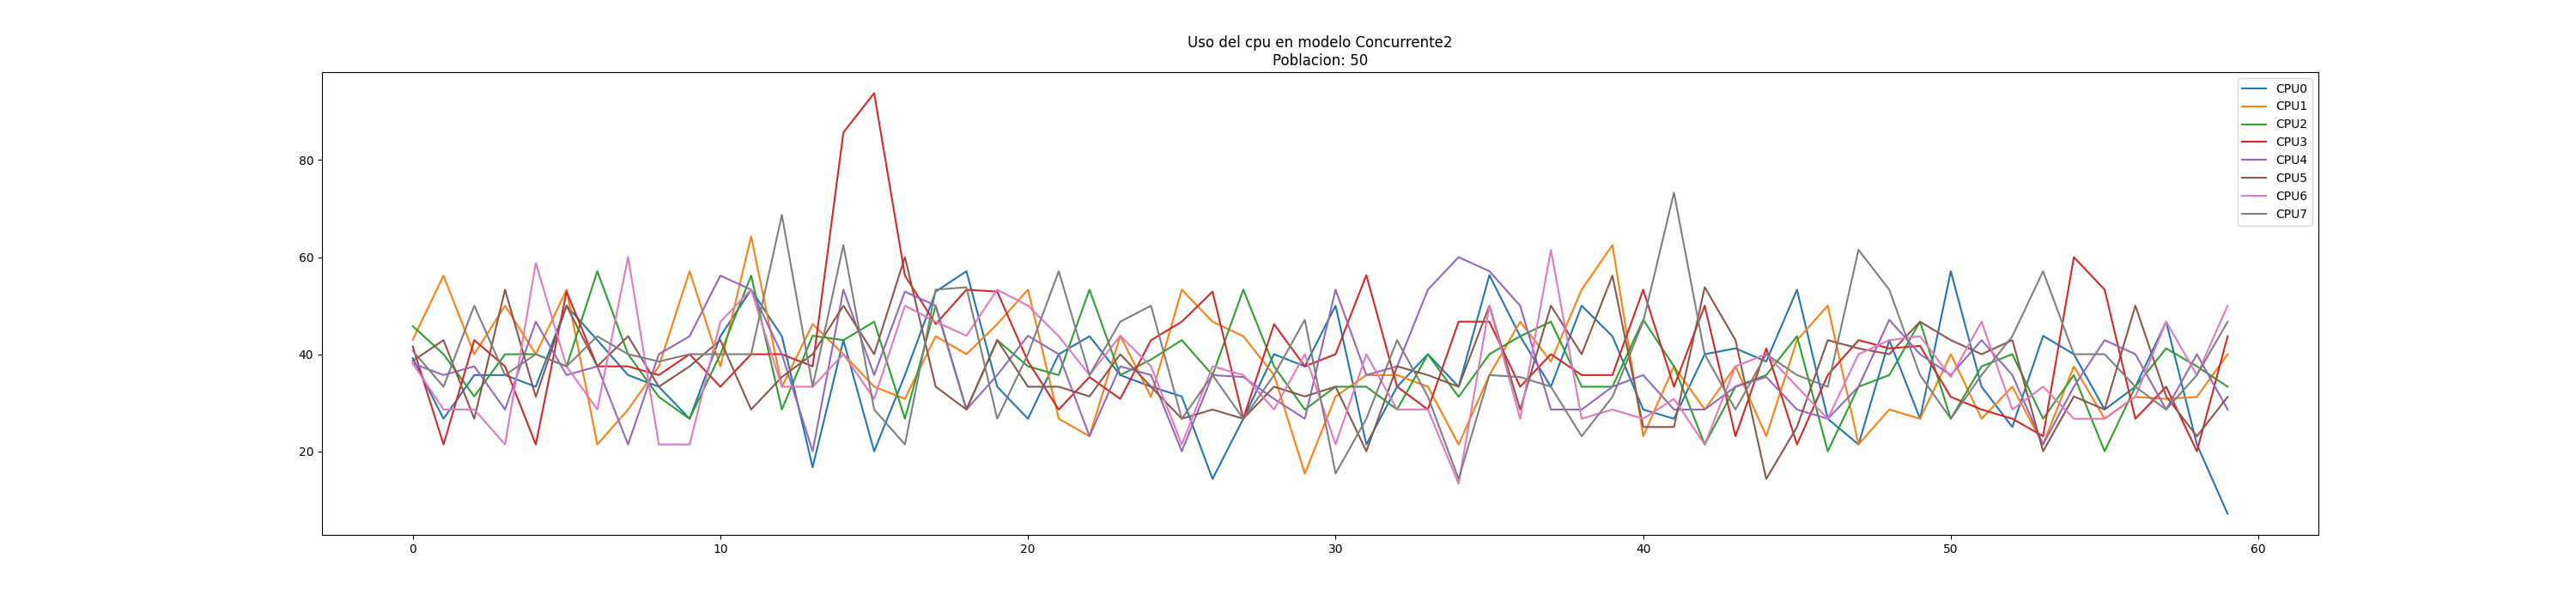
\includegraphics[width=\linewidth]{Plots/ModeloConcurrente2_Poblacion50.png}
    \caption{Uso de recursos de modelo Concurrente2 (4 procesos que se dividen la carga de creación de cromosomas)}
\end{figure}

\subsection{Ejemplo de ejecución}
A continuación se presenta un ejemplo de la ejecución descrita en el documento, que consta en una comparación de los cuatro modelos para Lorem Ipsum parcial (1000 letras) y completo (95500 letras)
\begin{center}
    

{\scriptsize

\begin{verbatim}
##################################################
Comparación con el texto parcial de longitud 1000
##################################################
Poblacion: 8, Iteraciones: 500
Secuencial:
Tiempo 0.31	 String: ¡OJvRinz,HhNxPSdakwUtñepQGjFXWM szbrfBKZAbIcuVt.om	 Error:973
Tiempo 0.42	 String: AEfdEJxShHBbdwTiyXsstPCPFkwenQBrFYJñtIMSmqpÑRIAUoq	 Error:862
Tiempo 0.54	 String: xaÑcMQhxrmjodslZEpsatBwmjeDaMFFblCbrtAÑVJtyfrVWDpt	 Error:757
Tiempo 0.64	 String: FrqCdVKxsuzTdLlkWusitllmx.,jlwLsZÑRUtkLJ¡wggÑ DiIl	 Error:664
Tiempo 0.76	 String: pf!fvFsysuDMdGlIYfsit,AmFC,IloOsptXettpYÑKgae cixw	 Error:587
Tiempo 0.87	 String: Jja¡,mzpsux¡dBlnCtsitbXmJY, loOsSnsethw,ANOdXAciXw	 Error:509
Tiempo 0.97	 String: ÑrrEoNopsuendBlgZdsit ¡mjt, qoes,ctettQaaGO,lCciQl	 Error:439
Tiempo 1.08	 String: LorZCgFpsukmdXl i.sit Ñmrt, loEsectet¡voafYKgecitL	 Error:377
Tiempo 1.19	 String: Lorem lpsuR d¡l!XXsit Ummt, zogsectetfKyakilmpciAg	 Error:328
Tiempo 1.29	 String: Lorem ñpsuG dvlñjJsit smpt, foIsectet jiaAikxvciqg	 Error:284
Concurrente1:
Tiempo 1.51	 String: bñJIdoCfMrPaAfRuSG,OFk.T!Vjtx gmWUWsQYlkicpnHzDKNE	 Error:977
Tiempo 2.33	 String: nzrpdlys¡m!kKlOTj,ZJHZKvPRlmZxnfScDbhuV SRJzjMJTaL	 Error:864
Tiempo 3.20	 String: oXrEkPcUKlwWQolol,jyFzivN.BicAn.ñctKIuV aiJ.puNaZk	 Error:768
Tiempo 4.17	 String: H.rBñIIDqKIWJolor!VWtwwyIAnDc!nULctNBua ahULFVQ,q.	 Error:672
Tiempo 5.04	 String: fmrjX,vVqLv.molorsm.t wPnHxHcjnwcctKtuJ azViyGcVRW	 Error:583
Tiempo 5.99	 String: ZhremS JsncWdolorodht bmutPYconDÑctKtu  aVHVifcK,J	 Error:492
Tiempo 6.88	 String:  urembdtsnnRdolorFzit Kmmt.rconbsctRtud awC iscjZg	 Error:420
Tiempo 7.74	 String: pKremtT¡sqlydolorSWit Lmxt,RconUQctetuI aMVgiscVrg	 Error:355
Tiempo 8.62	 String: VRremQR.sOzbdolorqÑit Zmct,wconp ctetuc a ipiscTrg	 Error:310
Tiempo 9.56	 String: JoremCPVsul dolorqUit ZmPt,ñconY!ctetue agipiscDGg	 Error:268
Concurrente2:
Tiempo 10.49	 String: qaPLdirJ SmrelÑolUEgxFuÑsbnqvBQsm,zxUpYAWKOiTuTZjD	 Error:972
Tiempo 11.40	 String: bfcemWbjPrmAxgvo.NvoSuKDjdaNiUiPFXo,tDIe qZpwSVHEH	 Error:858
Tiempo 12.33	 String: ,Rkem,cXwumYmMoorWLbtpuztGWSvTuUKccetTrQjE¡pGvsKgN	 Error:768
Tiempo 13.40	 String: lJsemniLNumVdoIorM!ñt yeAzROkon¡Mctet rDIdLpIUKPGT	 Error:656
Tiempo 14.40	 String: ZememmibRumÑdoboreu.t ieztozxon ectetñr,JdepIUeiTp	 Error:569
Tiempo 15.35	 String: pTremiip¡umWdolorNsht aeYt  ConOectetIrOÑdNpsh!i s	 Error:486
Tiempo 16.30	 String: ¡qremAipNumcdolorwsZt amktU VongectetkrNwdrpsQsisg	 Error:415
Tiempo 17.30	 String: OBremKipdumIdolorwsgt amet, donDectetRr BdUpESKi,g	 Error:363
Tiempo 18.39	 String: qWrem ipYumYdolorFsRt amet, wonsectettr UdgpsOeing	 Error:309
Tiempo 19.58	 String:  krem ipOum dolorgsnt amet, gonsectetur OdDpLxFing	 Error:266
Pool:
Tiempo 20.66	 String: rVgHes,FOCfBWXnlG RAcgMUSÑqD¡KxJpUuhaviQa!NyLñsmdg	 Error:972
Tiempo 21.73	 String: bZtVUjiMMZÑWA.lDj jYMuÑwOg,iñjnioñtwDuñña!cyAFvxwg	 Error:855
Tiempo 22.64	 String: KFres imBuSUWhlkP hQMH,!lB, WNnaFRtZtuNHaXWQLGcvpg	 Error:754
Tiempo 23.49	 String: l rev ipzuQLr,lVA SirWaf!k, conZeRt auGDaAdpGñceIg	 Error:668
Tiempo 24.39	 String: J!reh ipsuDUOclor ÑiaCaFg , congeOtCtuoaamWpfscRzg	 Error:583
Tiempo 25.25	 String: Bqrem ipsuoudolor xitoagrO, congeVtoturvaWiptschBg	 Error:502
Tiempo 26.29	 String: KYrem ipsuRgdolor sitAaQY , conYejteturJañipCscMng	 Error:438
Tiempo 27.20	 String: COrem ipsusEdolor sitcazEC, conKe¡teturgajipBscing	 Error:381
Tiempo 28.10	 String: oÑrem ipsumTdolor sitJalei, conñeWteturTakiphscing	 Error:327
Tiempo 29.00	 String: nDrem ipsumIdolor sit afek, conÑeXteturdadip!scing	 Error:276

Secuencial: 1.145	 Concurrente1: 8.975
Concurrente2: 10.174	 Pool: 9.246 
 **************************************************
Poblacion: 20, Iteraciones: 500
Secuencial:
Tiempo 30.72	 String: EH.CgRÑpOJjAVZIsñ!mJflTLwMnKzcXB,vkpueWi¡xyqSDxhGY	 Error:971
Tiempo 31.02	 String: Boes,GCpPGXxjil,NlMyr SFet,LzfNGextCnasVTdkpxsRTD!	 Error:816
Tiempo 31.31	 String: LoreukupqdRMjElo,iggk OZet, coEsectyAu,FadYpFscYJf	 Error:682
Tiempo 31.58	 String: LoregHkps!q SFloxbcVR rKet, coysectoSuQkadxpfscTnX	 Error:556
Tiempo 31.85	 String: LoremmipsEK dÑloiYpiB Bcet, coysecteiutIaddp.scing	 Error:459
Tiempo 32.12	 String: Lorem,ipsCm dPlosM,iV ycet, coqsecteñuTEadkpJscing	 Error:367
Tiempo 32.38	 String: LoremTipsVm deloN!NiQ abet, coVsecteeuGhadzpJscing	 Error:290
Tiempo 32.64	 String: LoremFipsvm dtlopysit aMet, coIsecteSuBHadHpÑscing	 Error:219
Tiempo 32.91	 String: Lorem ipsNm dqloNksit azet, coksecteVubvadTp¡scing	 Error:157
Tiempo 33.17	 String: Lorem ipsfm dÑloJLsit aget, consecteBuSfadQp,scing	 Error:108
Concurrente1:
Tiempo 33.53	 String: hUjÑ!hdjsvFGdfwLcXTyriaJknqDgZP VWHaAWO¡ tebFPmiAM	 Error:971
Tiempo 36.75	 String: oIkjqvHGspmFd!,ISbyhtVaXphQ gdplGcaexLyKVdVbBBMiRi	 Error:804
Tiempo 40.17	 String: cgbwZgqIswmLdlWvSmYwt aIOaV p meMceetBLPUdiRWsIiCe	 Error:672
Tiempo 43.49	 String: !wlyHMipsum dxWoc!sZt amvsP Oo mGcHetLpcIdihssjiÑg	 Error:543
Tiempo 46.83	 String: zocpf ipsum domorbsOt amjgG yohB,cletVfBpdiQnsciLg	 Error:432
Tiempo 50.02	 String: RoryJ ipsum dozorGs t amQtv xonpÑc,etCaoadipisciOg	 Error:336
Tiempo 53.21	 String: NorJm ipsum dolor sBt amRt, XonNhcCetvrw,dipisciBg	 Error:265
Tiempo 56.61	 String: Lorem ipsum doNor sit amot, SonLgcGetirmadipiscibg	 Error:198
Tiempo 60.07	 String: Lorem ipsum dolor sit amJt, IonsNcyet,rYadipiscing	 Error:146
Tiempo 63.84	 String: Lorem ipsum dolor sit am.t, gonsNcsetur adipiscing	 Error:106
Concurrente2:
Tiempo 67.52	 String: XqKaVo e,.LlEuUWhwGYd¡HsnñMQTcFDpKJNzxUbftBigjvRAS	 Error:972
Tiempo 69.20	 String: NFLeKahkouiMCruLbuñiEDÑe¡XM.ñBkMBH!esTvp uvP!XXiHb	 Error:823
Tiempo 70.80	 String: PIheoRjCsuAJcTemxvXitlEwJLKfjXCmCEgef GGZdcydsoin!	 Error:695
Tiempo 72.28	 String: Loueb CjsuXIuTe rKyit DIeWñecsdsqBReyñnG.dñPascing	 Error:579
Tiempo 73.68	 String: Lofef ipsuIRrxnurOsit kGeStXcoysPIneTñuÑAdzXyscing	 Error:474
Tiempo 75.08	 String: Lo,eu ipsuzWcoAJr sit ahetmFcoCsewqeBAZGadzNRscing	 Error:385
Tiempo 76.57	 String: Lore  ipsuvOÑooor sit ametMSconseu!eajL adeCRscing	 Error:306
Tiempo 77.92	 String: LoreM ipsun¡,ooor sit ametibconsej¡equn adnWfscing	 Error:242
Tiempo 79.32	 String: Loreu ipsuoHNolor sit ametcNconse.eeUuD adapZscing	 Error:183
Tiempo 80.63	 String: Lorem ipsuñbdolor sit amet, consecletuz adgp scing	 Error:132
Pool:
Tiempo 81.97	 String: .Kiloqfi!¡EhÑjgmMWT CHaPpO,qZXIkñcJvykxSUurvRAbwnG	 Error:969
Tiempo 83.66	 String: BSpFRiottÑSZnjGKduJie aejÑ,KGtnñecHtcui rdxYi.Linu	 Error:820
Tiempo 85.51	 String: LErhABipbuO,ZD,CrL!ieya.wd,HRinbecDYTuv zdiYigcing	 Error:675
Tiempo 87.41	 String: LHrWQuipsuvC!slVr,siXfapKK,oÑOnfecDgfua adiuigcing	 Error:555
Tiempo 89.16	 String: LNrWm ipouU gxlMrksiz ausT, esnXecynCuF adiIiAcing	 Error:449
Tiempo 90.97	 String: LorRm ipsuq ñzlorusit al!g, wBnsecTezuI adipiTcing	 Error:351
Tiempo 92.65	 String: Lorum ipsur sFlorpsit ayex, z nsecWeyuL adipidcing	 Error:272
Tiempo 94.39	 String: Lorym ipsum dolor,sit a¡ev, qÑnsectetun adipiscing	 Error:205
Tiempo 96.09	 String: Lorkm ipsum dolor sit amet, XnnsectetuJ adipiscing	 Error:148
Tiempo 98.12	 String: Lorhm ipsum dolorksit amet, .Lnsectetuq adipiscing	 Error:102

Secuencial: 2.732	 Concurrente1: 33.972
Concurrente2: 14.469	 Pool: 18.207 
 **************************************************
Poblacion: 200, Iteraciones: 500
Secuencial:
Tiempo 101.19	 String: dIHZYoAÑxfQRnVlgXrai,FK! ¡WBUES.,sVykMtjñOPkpbcuhJ	 Error:967
Tiempo 103.92	 String: LqrAEwRVSmvT floR Miu,Rmyy,FHFkN,sVmFÑrigU,pcscgnZ	 Error:711
Tiempo 106.64	 String: LLreYKiTXuVpBHlor vi  amsc, conp,cWzQurRaEÑpUscFng	 Error:502
Tiempo 109.25	 String: L!rednil!usXfflor Nit ammt, consvcUnmur adipBscUng	 Error:320
Tiempo 111.90	 String: Lsremwipsum¡Vllor Qit ammt, consecwevur adipdscing	 Error:182
Tiempo 114.51	 String: Lorem ipsum dÑlor Eit amet, consectetur adippscing	 Error:81
Tiempo 117.11	 String: Lorem ipsum dtlor sit amet, consectetur adipiscing	 Error:13
Tiempo 119.73	 String: Lorem ipsum dolor sit amet, consectetur adipiscing	 Error:3
Tiempo 122.22	 String: Lorem ipsum dolor sit amet, consectetur adipiscing	 Error:3
Tiempo 124.69	 String: Lorem ipsum dolor sit amet, consectetur adipiscing	 Error:3
Concurrente2:
Tiempo 127.26	 String: Vicvt,TGEKIqnFLrñZfyolxñFhnuyHkl.hvYDRc pDB!,KÑMdO	 Error:968
Tiempo 129.00	 String: LmÑQñmifñECO ¡l¡F.AitlhiTt,i,oe hqtN¡hi¡RdRpid HSa	 Error:712
Tiempo 130.76	 String: LWnuaYin,uW Qll¡pZ!itXAf¡t, qoBsUPtcqNrTkdNpisbJÑg	 Error:501
Tiempo 132.55	 String: LgqXWJizsuh ÑDloyeoit amEt, consmzteTnrTadNpiscbgg	 Error:333
Tiempo 134.54	 String: LotSm izsuY jKlorZgit amEt, consxdteturfaddpiscPwg	 Error:191
Tiempo 136.44	 String: Lo em iAsuM Rllor git amst, conseJteturLadipisc¡ng	 Error:86
Tiempo 138.23	 String: Lorem ipsum dolor sit amet, consectetur adipiscing	 Error:17
Tiempo 140.01	 String: Lorem ipsum dolor sit amet, consectetur adipiscing	 Error:3
Tiempo 141.82	 String: Lorem ipsum dolor sit amet, consectetur adipiscing	 Error:3
Tiempo 143.83	 String: Lorem ipsum dolor sit amet, consectetur adipiscing	 Error:3
Pool:
Tiempo 146.09	 String: CVywAPñbREXLpm!StIhDTSOQ.lGtzMZfeUrsxTigcBoJÑFqWNY	 Error:961
Tiempo 153.75	 String: LL.xi IñsZJqdwrPr MotW,vzsb Ñj!CecNktuSuadiGLwjiñz	 Error:701
Tiempo 160.98	 String: LCne¡ dQsum.dqypr sftFiYIFñ iUiqectetuCpadiw¡Ycing	 Error:494
Tiempo 168.23	 String: LmkeO VHsumNdolor sitfaCrvx hsnfectetur adinQscing	 Error:326
Tiempo 175.95	 String: Lorem iJsum dolor sitvaRetX consectetur adiniscing	 Error:183
Tiempo 183.94	 String: Lorem ipsum dolor sitnaIetÑ consectetur adipiscing	 Error:75
Tiempo 191.60	 String: Lorem ipsum dolor sit amet, consectetur adipiscing	 Error:8
Tiempo 199.43	 String: Lorem ipsum dolor sit amet, consectetur adipiscing	 Error:3
Tiempo 207.14	 String: Lorem ipsum dolor sit amet, consectetur adipiscing	 Error:3
Tiempo 214.81	 String: Lorem ipsum dolor sit amet, consectetur adipiscing	 Error:3

Secuencial: 26.077	 Concurrente1:  inf
Concurrente2: 18.697	 Pool: 76.385 
 **************************************************
Poblacion: 500, Iteraciones: 500
Secuencial:
Tiempo 223.42	 String: ¡ubW.f!jZQIHuKiiowUIwFPBdAñvTFDYrkSCgRknHÑ gACcscy	 Error:960
Tiempo 231.26	 String: tVrss PpTGñLO JXCzPR¡WñZmtbrwDUyf,Dathu!f KtzscJng	 Error:686
Tiempo 238.96	 String: LRrLK lp.uu¡!WvsizñAl akMtaFHSQaeDUQtursmlUxzscing	 Error:458
Tiempo 246.23	 String: LorXK ipMubktWlYrqñot amtt,khaslectqturjleLYiscing	 Error:263
Tiempo 253.30	 String: LorAi ipsumksSlor sit amxt,jToTsectetur aNRpiscing	 Error:117
Tiempo 260.05	 String: Lorem ipsum dolor sit amjt, consectetur adipiscing	 Error:20
Tiempo 266.63	 String: Lorem ipsum dolor sit amet, consectetur adipiscing	 Error:3
Tiempo 273.22	 String: Lorem ipsum dolor sit amet, consectetur adipiscing	 Error:3
Tiempo 279.75	 String: Lorem ipsum dolor sit amet, consectetur adipiscing	 Error:3
Tiempo 286.24	 String: Lorem ipsum dolor sit amet, consectetur adipiscing	 Error:3
Concurrente2:
Tiempo 292.88	 String: CqO D!bñelfJhULzATkpnSYzEPxH,.timrXgywIojGRcFK¡WMÑ	 Error:963
Tiempo 295.43	 String: btrVpEHoXSqrdjabrNkwtfhÑBt,ljoqJnxyMtQr vFipiYcmKf	 Error:678
Tiempo 298.01	 String: L,rmOyYpsZm dJBor  itoN!Yt,IdonVKufetLr qQifiscidM	 Error:438
Tiempo 300.53	 String: LdremRipsnm dflor ritkMmft, coniRGtetbr hqiniscinG	 Error:243
Tiempo 303.09	 String: Loremnipsum dolor !it¡dmet, consectetur adipiscing	 Error:109
Tiempo 305.67	 String: Loremgipsum dolor sit amet, consectetur adipiscing	 Error:19
Tiempo 308.20	 String: Lorem ipsum dolor sit amet, consectetur adipiscing	 Error:3
Tiempo 310.75	 String: Lorem ipsum dolor sit amet, consectetur adipiscing	 Error:3
Tiempo 313.31	 String: Lorem ipsum dolor sit amet, consectetur adipiscing	 Error:3
Tiempo 315.89	 String: Lorem ipsum dolor sit amet, consectetur adipiscing	 Error:3
Pool:
Tiempo 319.07	 String: VñvNKuodÑVSngWxtzDApiQbñsxpi!wj,qZHmESfTRDyldsbcIC	 Error:962
Tiempo 337.73	 String: ÑTrORpohsymhdYeXI TmzOamwtñnwMRje,LVt nMVdipesnQWz	 Error:679
Tiempo 356.48	 String: LtrPJdipsumTdaleg wi,BametoiKññÑet!ftqoQVdipeszcsl	 Error:446
Tiempo 374.83	 String: Lorem ipsumjdolJJ siw amet, zqmdectñtIibadipisdKqg	 Error:259
Tiempo 392.92	 String: Lorem ipsum dolo! sit amet, IoZsectetuZ adipiscidg	 Error:114
Tiempo 411.48	 String: Lorem ipsum dolor sit amet, consectetur adipiscing	 Error:18
Tiempo 430.16	 String: Lorem ipsum dolor sit amet, consectetur adipiscing	 Error:3
Tiempo 448.67	 String: Lorem ipsum dolor sit amet, consectetur adipiscing	 Error:3
Tiempo 466.94	 String: Lorem ipsum dolor sit amet, consectetur adipiscing	 Error:3
Tiempo 485.28	 String: Lorem ipsum dolor sit amet, consectetur adipiscing	 Error:3

Secuencial: 69.622	 Concurrente1:  inf
Concurrente2: 25.874	 Pool: 185.418 
 **************************************************
Poblacion: 1000, Iteraciones: 500
Secuencial:
Tiempo 505.45	 String: VsuDYdWkCuqvgOBBSwnoZJHxcUzQrRyNKmFeEgSjstjpf!zcKG	 Error:959
Tiempo 520.62	 String: LnukY ÑjsufxToGoG sie Fmeg,OvfVE mSekhx .Ejpiscynw	 Error:654
Tiempo 535.00	 String: LomAF I.sumtSo¡oP sit Mmet,oceAVlczetur UYQpiscing	 Error:406
Tiempo 549.01	 String: LoXem xasumGdolor sit amet, cfnsectetur ZdKpiscing	 Error:205
Tiempo 562.27	 String: Lorem ipsum dolor sit amet, consectetur Ñdipiscing	 Error:70
Tiempo 575.53	 String: Lorem ipsum dolor sit amet, consectetur adipiscing	 Error:3
Tiempo 589.00	 String: Lorem ipsum dolor sit amet, consectetur adipiscing	 Error:3
Tiempo 602.82	 String: Lorem ipsum dolor sit amet, consectetur adipiscing	 Error:3
Tiempo 616.10	 String: Lorem ipsum dolor sit amet, consectetur adipiscing	 Error:3
Tiempo 629.81	 String: Lorem ipsum dolor sit amet, consectetur adipiscing	 Error:3
Concurrente2:
Tiempo 643.54	 String: YDdLF¡FeUCRGMbznw ¡VuBtnzDwpl!oñGrEiAÑmaÑVcZQLcepO	 Error:961
Tiempo 647.16	 String: nCxGa hñELvWZAAop sztdamlm, ko.FgemNturEP oWi,ci,F	 Error:659
Tiempo 650.87	 String: RxHe  ipiÑy daXor sit amEw, ro.JlPtotur udiMiFcidg	 Error:412
Tiempo 654.50	 String: RZren ip!Ym do.or sit amet, co,sIctetur adiEiscitg	 Error:223
Tiempo 658.32	 String: Lorex ipsum doIor sit amet, consectetur adipiscing	 Error:78
Tiempo 662.11	 String: Lorem ipsum dolor sit amet, consectetur adipiscing	 Error:3
Tiempo 665.61	 String: Lorem ipsum dolor sit amet, consectetur adipiscing	 Error:3
Tiempo 669.39	 String: Lorem ipsum dolor sit amet, consectetur adipiscing	 Error:3
Tiempo 672.99	 String: Lorem ipsum dolor sit amet, consectetur adipiscing	 Error:3
Tiempo 676.72	 String: Lorem ipsum dolor sit amet, consectetur adipiscing	 Error:3
Pool:
Tiempo 681.49	 String: URDoeAUiRBÑQOHEr,qslpTEVISDKzzfawcAYsNkahgxñ,BZyFZ	 Error:962
Tiempo 716.31	 String: UOyMvaNuvuqlH.plrOsdJ aQet,,ayFnYcBfF,r xiimisccvg	 Error:654
Tiempo 750.93	 String: LdcAWPumsuQrdokirIsit aLet,Ñ Mfs clJcur ydiyiscing	 Error:407
Tiempo 785.73	 String: LopemTJWsuw doxHr sit aDet, uonsMctUtur adiwiscing	 Error:203
Tiempo 819.91	 String: Lorem,ipsuU dolor sit amet, consRctetur adipiscing	 Error:64
Tiempo 854.04	 String: Lorem ipsum dolor sit amet, consectetur adipiscing	 Error:3
Tiempo 888.04	 String: Lorem ipsum dolor sit amet, consectetur adipiscing	 Error:3
Tiempo 923.18	 String: Lorem ipsum dolor sit amet, consectetur adipiscing	 Error:3
Tiempo 957.23	 String: Lorem ipsum dolor sit amet, consectetur adipiscing	 Error:3
Tiempo 991.55	 String: Lorem ipsum dolor sit amet, consectetur adipiscing	 Error:3

Secuencial: 138.363	 Concurrente1:  inf
Concurrente2: 37.217	 Pool: 344.774 
 **************************************************
##################################################
Comparación con el texto completo de longitud 92551
##################################################
Poblacion: 8, Iteraciones: 500
Secuencial:
Tiempo 1026.42	 String: ,NñhUYMzTJTCq SgqLsXRd¡tbWBPF.HljfGxw!aÑVInyimQedñ	 Error:90780
Tiempo 1038.18	 String: LnOBPxJpkmVA!TVyv sqXÑxitjoXSjmf BKzGZk aMLHiIN!m!	 Error:83304
Tiempo 1049.49	 String: LtSokEnpMuzzRiEoE sihNyMeD!IMwiKony,slZ ayepiulYWs	 Error:76502
Tiempo 1060.61	 String: LñtVeGipvuEoNMaoa si!UCfeQ,SKRa,SWNeScr aOhpislmkM	 Error:70259
Tiempo 1072.02	 String: LqOPi.ipsudUZ.ooP siGbaCeE,ZNsRPSK etyr asjpisÑrjU	 Error:64559
Tiempo 1083.23	 String: L,Lgtñipsun V lor sicOaGeZ,GcoysbHKetñr agZpiswinW	 Error:59324
Tiempo 1093.99	 String: LCXGDLipsuI GClor siwKayes,scoesprbetbr adspis,inQ	 Error:54356
Tiempo 1104.16	 String: LQHgmjipsui dolor siKxa,eD, coVsYyUetur adIpisqinO	 Error:50025
Tiempo 1114.32	 String: Lw emdipsuC dolor siñgaGeV, coOserUetur ad¡pisZing	 Error:45954
Tiempo 1124.86	 String: LXDemvipsui dolor sibAameQ, coqseCTetur adQpisbing	 Error:42164
Concurrente1:
Tiempo 1135.98	 String: FfzDR WrNZRjdYIsAEmcUehBOutJ.ylN!n.wHEXaP!yKkgoñLG	 Error:90803
Tiempo 1139.42	 String: L!¡Gr bnqanbd¡evoVJQCcKSeHyJ¡jlWñW,bIvf ad!¡xx¡GGe	 Error:83388
Tiempo 1142.83	 String: LZurs S,ABg.dohmpLlGFNFAeebTixNcCOWeu.A adZbfPFiCR	 Error:76705
Tiempo 1146.70	 String: LJlew twO!uwdoE z uDzuv etg PFc ehtetfy adlrqjgiCc	 Error:70180
Tiempo 1150.30	 String: LAJeE tUdÑu dociK PvO Qhet. ñZjQeStetpT adxN QdiUp	 Error:64486
Tiempo 1153.89	 String: L pem jwuud dohJg Mrw bketP LñcpeLtetdj ady!VZciEg	 Error:59303
Tiempo 1157.47	 String: LpQem IpRum doxGT Iym JGetP c.jpeFtetmv adpCixciqg	 Error:54357
Tiempo 1161.01	 String: LbTem Wpxum doyEY bo! eVetV cjEfeOtetJT adBviMciog	 Error:49979
Tiempo 1164.51	 String: LAQem apxum docBU UOv INetJ cDaneXtetCu ad!piBciRg	 Error:45679
Tiempo 1167.95	 String: LtVem opLum domFM oMK NZetz ceykegtetwk adipibcing	 Error:42051
Concurrente2:
Tiempo 1171.91	 String: gñikrsqB!nbYjytjJvAFMmeAoXf,zxTaZt.whU,¡GdqDHQWDÑS	 Error:90744
Tiempo 1175.54	 String: MBWZvjXRL CwIzlaUL fuuBsYlvkUovehCMt.nr.DdPDTGCgZÑ	 Error:83288
Tiempo 1179.12	 String: doPAaG!.UjB¡X!lutDH.FGavdLÑrOoNsiVcK!brmNditn!v!nm	 Error:76198
Tiempo 1182.51	 String: SoQeILZYqOerdVlZSvslABaS¡¡iWkonsTsNpÑlr UdiVJZQPnñ	 Error:69922
Tiempo 1185.80	 String: ao¡ed TYÑÑWxdyl!UOsTTÑaB RÑbVonshxtebZr adipygTxnk	 Error:64236
Tiempo 1189.13	 String: DoEeV USs,mBdsljdRsÑomanYQTpUonsystemzr adip BDnni	 Error:59343
Tiempo 1192.50	 String: no eb I sEm dclikgsV.zayHdEILonsMpteWtr adiph.Ninv	 Error:54311
Tiempo 1196.06	 String: woVel OYsum dNlNFmsij aVxtFtsonsFgtetOr adipItSinK	 Error:49776
Tiempo 1199.68	 String: Yosem nWsum dglRrhsik ayYtñTHons.Otet¡r adiphXQint	 Error:45691
Tiempo 1203.39	 String: ,oÑem Mnsum dflWrlsiC avgtn¡uonslptetPr adipsIpinb	 Error:41922
Pool:
Tiempo 1207.49	 String: uv,DE!iolKeUBñGpqmNdJCgzRcIkaPTbjxMfOrSLhJYVyÑw HZ	 Error:90776
Tiempo 1218.93	 String: wvJnujiFXY,ñEVlyr sjt HVuqUmyimPPNJ t,nLmHMOoHCvTg	 Error:83477
Tiempo 1230.16	 String: Wo!bQpitWQbXqblTr sOt aFURguxzDVxYfYtiÑtnIñ.bÑqzog	 Error:76460
Tiempo 1241.04	 String: LoWLdciXsEsZdBlOr sUt aGuxÑTpMKMÑcZetBAOdeSD dvlDg	 Error:70223
Tiempo 1252.77	 String: LofV! iEsHmDdylWr sFt auMxlatLDZfcOet¡g.tgo!ÑÑrOVg	 Error:64357
Tiempo 1264.26	 String: LoW . issMm d.lJr s t amJ!nhzij!QcBetVÑXKXiUlnmfUg	 Error:58881
Tiempo 1276.00	 String: LoOiN iMsDm dQlOr snt ami CrEEndYcFetE.AQdieiORefg	 Error:53854
Tiempo 1287.22	 String: LoDVV iQsfm dVlbr sVt amdIWRaundWcRetcBzbdiiizcuPg	 Error:49411
Tiempo 1298.18	 String: LoRFu iwstm dslor sht amPXb ñznRncdetstpqdieidczqg	 Error:45278
Tiempo 1309.52	 String: LoioG ifsvm djlor sYt amlVg xonshcÑetn,aCdiiiBcEtg	 Error:41482

Secuencial: 109.737	 Concurrente1: 35.921
Concurrente2: 35.394	 Pool: 113.169 
 **************************************************

\end{verbatim}}
\end{center}


\twocolumn




\begin{thebibliography}{X}

% libros

\bibitem{Genéticos} \textsc{Montana, David J. y Lawrence Davis (1989).} (Training Feedforward Neural Networks Using Genetic Algorithms).Proceedings of the 11th International Joint
Conference on Artificial Intelligence - Volume 1 . IJCAI’89. Detroit, Michigan:
Morgan Kaufmann Publishers Inc., págs. 762-767. URL:
dl.acm.org/citation.cfm?id=1623755.1623876.



\bibitem{} \textsc{D. Dervis Karaboga(2005)} (An Idea Based On Honey Bee Swarm for Numerical Optimization), Technical Report-TR06, Erciyes University, Engineering Faculty, Computer Engineering Department .

\bibitem{hormigas} \textsc{Robles Algarin, Carlos Arturo(2011)}(Optimización por colonia de hormigas: Aplicaciones y tendencias).Universidad Cooperativa de Colombia - Universidad del Magdalena


\bibitem{BS} \textsc{Cuevas, Erik. Ortega-Sánchez, Noé(2011)} (El algoritmo de búsqueda armónica y su uso en el procesamiento digital de imágenes)Departamento de Electrónica, Universidad de Guadalajara, CUCEI, Guadalajara, Jalisco, México











\end{thebibliography}
\end{document}

